\section{Additional Generalization Diagnostics}

Figure~\ref{fig:appendix-gap} answers two distinct overlap questions using the collections of peptide pairs that share presenting restriction and parent protein (pair pools) from \plainMatchedOOF{} under research question 4 (RQ4). The upper panel reports, for each \plainHLA{} gene group or \plainHtwo{} restriction, the mean AUROC change across tissue--antigen-presenting-molecule combinations (mean task AUROC change) after exact peptides are separated across all combinations (tasks); zero means no mean change and a negative bar means lower performance under \plainPeptideOOF{}. The lower panel reports the mean percentage of unique held-out parent proteins that also occur in the fitting partition. A nonzero lower-panel bar therefore shows residual protein identity overlap and demonstrates that \plainPeptideOOF{} does not prevent parent-protein overlap (\plainProteinDisjoint{}). The \plainMatchedOOF{} reference is not the separate \plainFixedTest{}.

\begin{table}[htbp]
\centering
\caption{Statistics comparing the same biological combinations under ordinary and peptide-separated evaluation (within-task paired statistics). Differences are \plainPeptideOOF{} minus \plainMatchedOOF{}. The numbers of tissue--antigen-presenting-molecule combinations with positive, tied, and negative differences (\plainWtl{}) are reported; confidence intervals are based on 10,000 resamples of complete biological combinations (task resampling); \(q_{\mathrm{BH}}\) adjusts eight Wilcoxon tests. This is a downstream statistical analysis, not an additional data split.}
\label{tab:paired-stats}
\small
\setlength{\tabcolsep}{1pt}
\textbf{Human}\par\smallskip
\begin{tabular}{lrrrlll}
\toprule
Metric & Mean & Median & \shortstack{Median-shift\\estimate (HL)} & \shortstack{Positive/tied/negative\\task counts (W/T/L)} & 95\% CI & BH $q$ \\ 
\midrule
AUROC & -0.0628 & -0.0484 & -0.0552 & 12/0/145 & [-0.0728, -0.0534] & $1.29\times10^{-22}$ \\ 
AUPRC & -0.0691 & -0.0509 & -0.0621 & 10/0/147 & [-0.0799, -0.0588] & $1.29\times10^{-22}$ \\ 
Accuracy & -0.0625 & -0.0455 & -0.0563 & 17/2/138 & [-0.0727, -0.0529] & $2.12\times10^{-22}$ \\ 
MCC & -0.1249 & -0.0907 & -0.1125 & 18/0/139 & [-0.1453, -0.1057] & $2.12\times10^{-22}$ \\ 
\bottomrule
\end{tabular}
\par\medskip
\textbf{Mouse}\par\smallskip
\begin{tabular}{lrrrlll}
\toprule
Metric & Mean & Median & \shortstack{Median-shift\\estimate (HL)} & \shortstack{Positive/tied/negative\\task counts (W/T/L)} & 95\% CI & BH $q$ \\ 
\midrule
AUROC & -0.0863 & -0.0832 & -0.0859 & 2/0/22 & [-0.1106, -0.0632] & $6.81\times10^{-7}$ \\ 
AUPRC & -0.0994 & -0.1040 & -0.1002 & 2/0/22 & [-0.1293, -0.0706] & $1.67\times10^{-6}$ \\ 
Accuracy & -0.0918 & -0.0804 & -0.0902 & 1/0/23 & [-0.1207, -0.0652] & $4.77\times10^{-7}$ \\ 
MCC & -0.1838 & -0.1632 & -0.1802 & 1/0/23 & [-0.2415, -0.1306] & $4.77\times10^{-7}$ \\ 
\bottomrule
\end{tabular}
\end{table}

\begin{figure}[htbp]
\centering
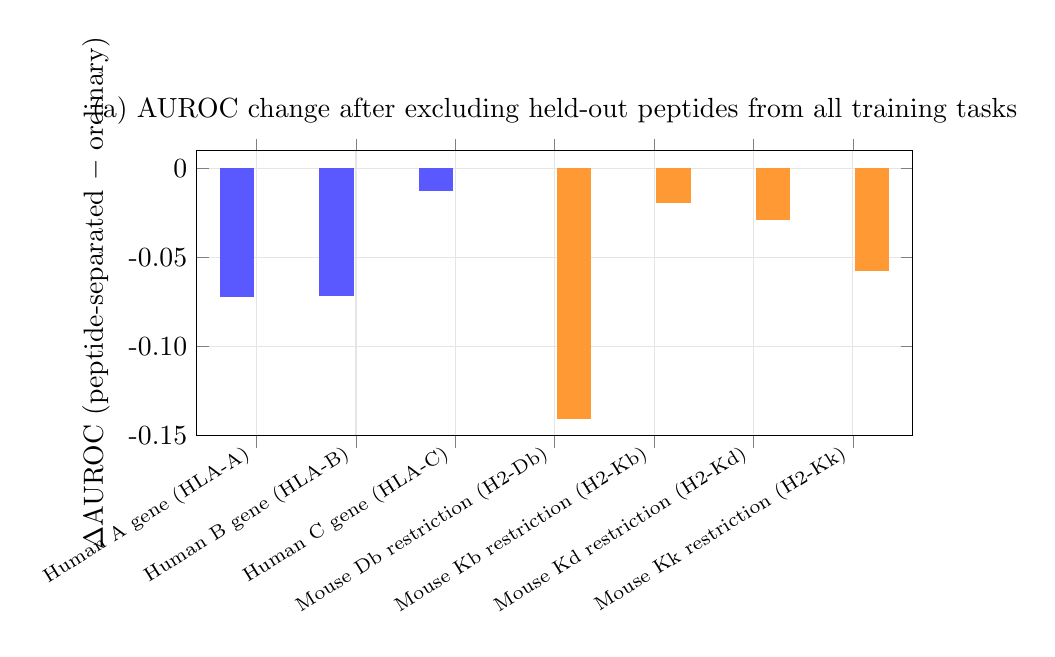
\begin{tikzpicture}
\begin{axis}[
    width=0.88\linewidth,
    height=5.2cm,
    ybar,
    bar width=12pt,
    title={(a) AUROC change after excluding held-out peptides from all training tasks},
    ymin=-0.15,ymax=0.01,
    ytick={-0.15,-0.10,-0.05,0},
    yticklabels={-0.15,-0.10,-0.05,0},
    symbolic x coords={HLA-A,HLA-B,HLA-C,H2-Db,H2-Kb,H2-Kd,H2-Kk},
    xtick={HLA-A,HLA-B,HLA-C,H2-Db,H2-Kb,H2-Kd,H2-Kk},
    xticklabels={Human A gene (HLA-A),Human B gene (HLA-B),Human C gene (HLA-C),Mouse Db restriction (H2-Db),Mouse Kb restriction (H2-Kb),Mouse Kd restriction (H2-Kd),Mouse Kk restriction (H2-Kk)},
    x tick label style={rotate=32,anchor=east,font=\scriptsize},
    ylabel={$\Delta$AUROC (peptide-separated $-$ ordinary)},
    grid=major,
    grid style={gray!20}
]
\addplot+[fill=blue!65,draw=blue!65] coordinates {(HLA-A,-0.0718) (HLA-B,-0.0712) (HLA-C,-0.0122)};
\addplot+[fill=orange!80,draw=orange!80] coordinates {(H2-Db,-0.1404) (H2-Kb,-0.0192) (H2-Kd,-0.0284) (H2-Kk,-0.0571)};
\end{axis}
\end{tikzpicture}

\vspace{0.7cm}

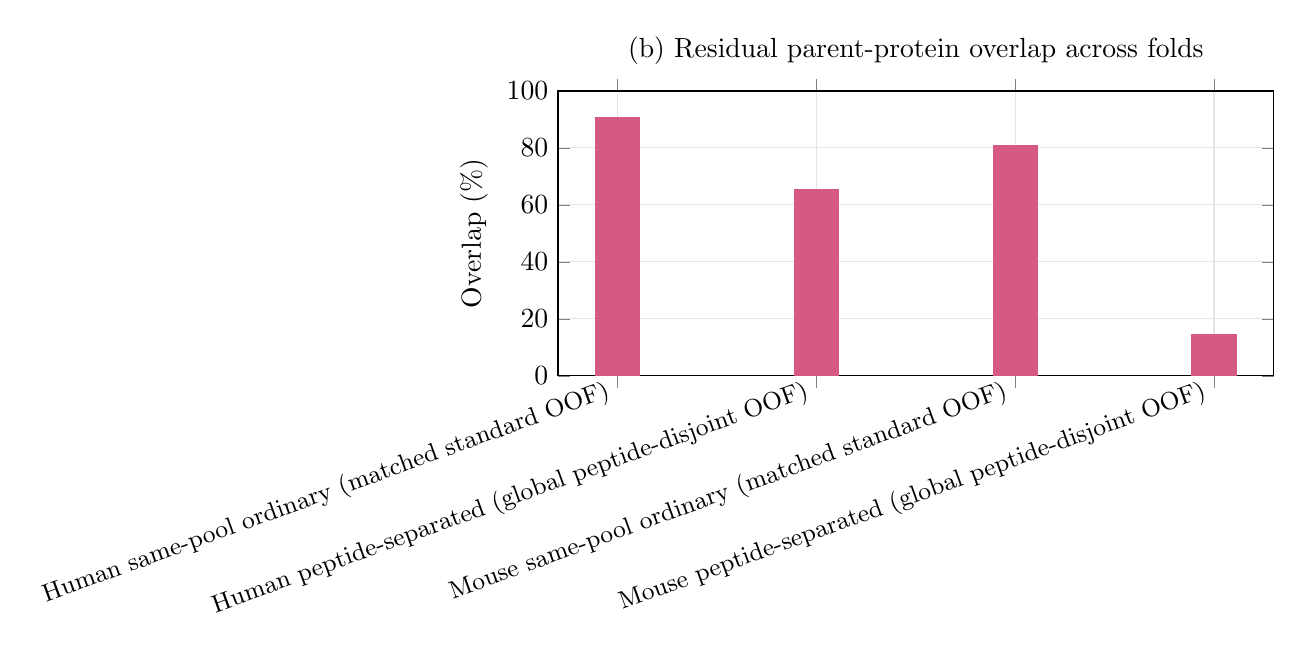
\begin{tikzpicture}
\begin{axis}[
    width=0.88\linewidth,
    height=5.2cm,
    ybar,
    bar width=16pt,
    title={(b) Residual parent-protein overlap across folds},
    ymin=0,ymax=100,
    symbolic x coords={Human matched,Human global,Mouse matched,Mouse global},
    xtick=data,
    xticklabels={Human same-pool ordinary (matched standard OOF),Human peptide-separated (global peptide-disjoint OOF),Mouse same-pool ordinary (matched standard OOF),Mouse peptide-separated (global peptide-disjoint OOF)},
    x tick label style={rotate=20,anchor=east,font=\small},
    ylabel={Overlap (\%)},
    grid=major,
    grid style={gray!20}
]
\addplot+[fill=purple!65,draw=purple!65] coordinates {(Human matched,90.64) (Human global,65.26) (Mouse matched,80.69) (Mouse global,14.37)};
\end{axis}
\end{tikzpicture}
\caption{Generalization diagnostics based on \plainMatchedOOF{}. (a) Task-mean \plainPeptideOOF{} minus \plainMatchedOOF{} AUROC by \plainHLA{} gene group or \plainHtwo{} restriction; negative values indicate lower performance after exact peptide separation. (b) Mean fraction within each fold of unique held-out parent proteins also observed during fitting; nonzero values quantify residual protein overlap.}
\label{fig:appendix-gap}
\end{figure}

\section{Detailed Model Comparisons When Held-out Peptides Are Absent from All Training Tasks}

\begin{table}[htbp]
\centering
\caption{Selected AUROC comparisons between models evaluated on the same biological combinations and folds (paired AUROC comparisons) under \plainPeptideOOF{}, using identical folds built from transitively linked peptide pairs (connected-component folds). Differences place the first model minus the second; intervals are based on 10,000 resamples of complete biological combinations (task resampling), and \(q\) values are adjusted for multiple testing within the species--metric family (BH-FDR adjusted).}
\label{tab:appendix-strict-paired}
\scriptsize
\setlength{\tabcolsep}{0.8pt}
\textbf{Human}\par\smallskip
\begin{tabularx}{\textwidth}{@{}>{\raggedright\arraybackslash}Xrrlll@{}}
\toprule
Comparison & Mean & Median & \shortstack{Positive/tied/negative\\task counts (W/T/L)} & 95\% CI & BH \(q\) \\
\midrule
TissuePMHC $-$ \plainSharedHeads{} & +0.0091 & +0.0095 & 118/0/39 & [0.0067, 0.0116] & $2.27\times10^{-11}$ \\
TissuePMHC $-$ \plainPlainDual{} & +0.0097 & +0.0081 & 122/0/35 & [0.0076, 0.0119] & $1.36\times10^{-14}$ \\
TissuePMHC $-$ \plainAuxDual{} & +0.0010 & -0.0008 & 76/1/80 & [-0.0008, 0.0029] & 0.442 \\
TissuePMHC $-$ \plainBLOSUM{} random forest & +0.0440 & -- & 149/0/8 & [0.0392, 0.0489] & $3.43\times10^{-26}$ \\
TissuePMHC $-$ one-hot & +0.0525 & -- & 157/0/0 & [0.0479, 0.0571] & $8.14\times10^{-27}$ \\
\plainAuxDual{} $-$ \plainPlainDual{} & +0.0087 & -- & 144/0/13 & [0.0074, 0.0100] & $3.02\times10^{-23}$ \\
\plainAuxDual{} $-$ \plainSharedHeads{} & +0.0081 & -- & 123/0/34 & [0.0058, 0.0103] & $3.30\times10^{-11}$ \\
\bottomrule
\end{tabularx}
\par\medskip
\textbf{Mouse}\par\smallskip
\begin{tabularx}{\textwidth}{@{}>{\raggedright\arraybackslash}Xrrlll@{}}
\toprule
Comparison & Mean & Median & \shortstack{Positive/tied/negative\\task counts (W/T/L)} & 95\% CI & BH \(q\) \\
\midrule
\plainMMoE{} $-$ \plainSharedHeads{} & -0.0008 & -0.0018 & 10/0/14 & [-0.0062, 0.0049] & 0.509 \\
\plainMMoE{} $-$ \plainBLOSUM{} random forest & +0.0023 & +0.0039 & 14/0/10 & [-0.0052, 0.0091] & 0.509 \\
\bottomrule
\end{tabularx}
\end{table}

\begin{table}[htbp]
\centering
\caption{Stability across separate \plainSeeds{} and benefit from averaging predictions under \plainPeptideOOF{} on folds built from transitively linked peptide pairs (connected-component folds). Gain is the AUROC after averaging predictions across \plainSeeds{} (ensemble AUROC) minus the mean AUROC of the separate runs.}
\label{tab:appendix-strict-seeds}
\footnotesize
\setlength{\tabcolsep}{2pt}
\begin{tabularx}{\textwidth}{>{\raggedright\arraybackslash}p{1.0cm}
                            >{\raggedright\arraybackslash}Xrrrr}
\toprule
Species & Model & Mean of separate \plainSeeds{} & \shortstack{Standard deviation across\\random initializations (seed SD)} & Prediction average (ensemble) & Gain \\
\midrule
Human & One-hot logistic regression & 0.7127 & 0.0000 & 0.7127 & 0.0000 \\
Human & \plainBLOSUM{} random forest & 0.7193 & 0.0006 & 0.7212 & +0.0019 \\
Human & \plainSharedHeads{} & 0.7313 & 0.0043 & 0.7561 & +0.0248 \\
Human & \plainPlainDual{} using an \plainMLP{} & 0.7394 & 0.0043 & 0.7555 & +0.0161 \\
Human & \plainAuxDual{} & 0.7503 & 0.0038 & 0.7642 & +0.0139 \\
Human & TissuePMHC & 0.7505 & 0.0007 & 0.7652 & +0.0147 \\
Mouse & \plainBLOSUM{} random forest & 0.7491 & 0.0012 & 0.7507 & +0.0016 \\
Mouse & \plainSharedHeads{} & 0.7327 & 0.0031 & 0.7538 & +0.0211 \\
Mouse & \plainMMoE{} & 0.7211 & 0.0027 & 0.7529 & +0.0318 \\
\bottomrule
\end{tabularx}
\end{table}

\clearpage
\section{Details of Tissue-blind General Presentation Controls}

\begin{table}[htbp]
\centering
\caption{Sensitivity analysis comparing the NetMHCpan \plainBA{} with its \plainEL{}. Both rankings are oriented so that larger scores indicate stronger predicted propensity.}
\label{tab:appendix-netmhcpan-el-ba}
\small
\setlength{\tabcolsep}{4pt}
\begin{tabularx}{\textwidth}{>{\raggedright\arraybackslash}p{1.0cm}
                            >{\raggedright\arraybackslash}Xrrr}
\toprule
Species & Evaluation & \plainBA{} AUROC & \plainEL{} AUROC & \plainEL{} $-$ \plainBA{} \\
\midrule
Human & \plainFixedTest{} & 0.6577 & 0.6833 & +0.0256 \\
Human & Complete training pool & 0.6559 & 0.6823 & +0.0264 \\
Mouse & \plainFixedTest{} & 0.6847 & 0.6893 & +0.0046 \\
Mouse & Complete training pool & 0.6778 & 0.6802 & +0.0024 \\
\bottomrule
\end{tabularx}
\end{table}

\begin{table}[htbp]
\centering
\caption{Combining scores using a rule learned on other folds (cross-fitted incremental stacking) with \plainGeneralPMHC{} whose external scores were \plainFrozen{}. The combined column uses the external score and the corresponding tissue-conditioned model score.}
\label{tab:appendix-general-stacking}
\footnotesize
\setlength{\tabcolsep}{3pt}
\begin{tabularx}{\textwidth}{>{\raggedright\arraybackslash}p{1.0cm}
                            >{\raggedright\arraybackslash}X
                            >{\raggedright\arraybackslash}Xrr}
\toprule
Species & Protocol & External control & External only & Combined \\
\midrule
Human & \plainFixedTest{} & MHCflurry predicted presentation & 0.6851 & 0.8453 \\
Human & \plainFixedTest{} & NetMHCpan \plainEL{} & 0.6833 & 0.8447 \\
Human & \plainPeptideOOF{} & MHCflurry predicted presentation & 0.6867 & 0.7693 \\
Human & \plainPeptideOOF{} & NetMHCpan \plainEL{} & 0.6740 & 0.7651 \\
Mouse & \plainFixedTest{} & MHCflurry predicted presentation & 0.6564 & 0.8565 \\
Mouse & \plainFixedTest{} & NetMHCpan \plainEL{} & 0.6893 & 0.8564 \\
Mouse & \plainPeptideOOF{} & MHCflurry predicted presentation & 0.6464 & 0.7564 \\
Mouse & \plainPeptideOOF{} & NetMHCpan \plainEL{} & 0.6420 & 0.7534 \\
\bottomrule
\end{tabularx}
\end{table}
